
The principle goal of spin-dependent SIDIS experiments is to perform flavor 
decomposition of nucleon spin structure taking advantage of flavor tagging. 
In this section, we first express the SIDIS cross sections and asymmetries at 
\lo (LO) and summarize the HERMES results of ``purity method'' (more details
 in Appendix). After introducing the \nlo cross sections, we 
 summarize the NLO global QCD analysis method. 
We will then outline new methods of flavor decomposition:
the Christova-Leader method at leading order and next-to-leading order.
Theoretical models
of polarized light sea asymmetry $\Delta \bar{u}-\Delta \bar{d}$ is summarized at the end.
Throughout this proposal, SU(2) isospin symmetry and charge conjugation invariance are  
assumed and heavy quark contributions are neglected.

\section{Semi-Inclusive DIS kinematic definitions}

\section{Beam-target double-spin asymmetries at \lo}
 At the leading order, the 
 SIDIS process is separated into a hard-scale quark scattering 
 followed by a soft-scale hadronization.
 The ``naive $x$-$z$ separation'' assumption, on which the SMC and HERMES
analysis were based, implies that the spin-independent 
($\sigma^{h}$)
and the spin-dependent ($\Delta \sigma^{h}$)
  cross sections follow: 
\begin{eqnarray}  
 \sigma^{h} (x,z) & = & \sum_{f} e_f^2 q_f(x) \cdot D_{q_f}^{h}(z),  \hspace{0.5cm}
 \Delta \sigma^{h} (x,z)  =  \sum_{f} e_f^2 \Delta q_f(x) \cdot D_{q_f}^{h}(z),  
\label{eq:fact}  
\end{eqnarray}  
where $x=Q^2/2M\nu$, $z=E_h/\nu$.
 The fragmentation functions $D_{q_f}^{h}(z)$ represent the probability that a quark
 $f$ fragments into a hadron $h$.  

Considering the beam and target polarization ($P_B$ and $P_T$),
 and the dilution factor ($f^h=\sigma_{pol. N}^h/\sigma_{all N}^h$), which accounts for
the unpolarized nucleons in the target, 
the double-spin asymmetry~\cite{hermesthesis} for a longitudinally polarized 
beam on a longitudinally polarized target is : 
% ($A_2^h \approx 0$)
\begin{equation}
A_{\parallel}^h =  f^h P_B P_T \cdot {\cal P}_{kin} \cdot A_{1N}^h, \\
\label{Eq:apara}
\end{equation}  
the kinematic factor ${\cal P}_{kin}$ is: 
\begin{equation}
{\cal P}_{kin}  = {\cal D} \cdot (1+ \gamma \eta) 
\cdot { 1+R \over 1 + \gamma^2 }, \\
\label{Eq:pkin}
\end{equation}  
in which
\begin{eqnarray}
%y &= & \nu / E_0, \hspace{1.0cm} \gamma^2 = {Q^2 / \nu^2}, \hspace{1.0cm} R =  \sigma_L / \sigma_T, \nonumber \\
\eta &= & {2 \gamma (1-y) \over 2-y }, \hspace{2.0cm} {\cal D} =  {1-(1-y) \epsilon \over 1+ \epsilon \cdot R }, \nonumber \\
\epsilon^{-1} & = & 1+ 2 ( 1 + {\nu^2 /Q^2} ) \tan^2({\theta_e / 2}),
\end{eqnarray}
 ${\cal D}$ is the virtual photon polarization,
$R(x, Q^2) =  \sigma_L / \sigma_T$ accounts for the 
longitudinal component of the virtual photon 
%which has been assumed to be the same for semi-inclusive and the inclusive cases, 
and $y =  \nu / E_0$, 
$\gamma^2(x,Q^2) = 4 M^2 {x^2 / Q^2}$. 
In the current fragmentation regime, 
%the leading hadron from the fragmentation
%is correlated with the struck quark, 
the virtual photon asymmetry  
is defined as: 
\begin{equation}
A_{1N}^h(x,Q^2,z)  \equiv {\Delta \sigma^h(x,Q^2,z) \over \sigma^h(x,Q^2,z)}={\sum_{f} e_f^2 \Delta q_f(x,Q^2) \cdot D_{q_f}^{h}(z,Q^2) \over \sum_{f} e_f^2 q_f(x,Q^2) \cdot D_{q_f}^{h}(z,Q^2)}.
\label{Eq:a1h}
\end{equation} 
Each individual measurement on $A_{1N}^h(x,Q^2,z)$ provides an independent constrain on the polarized parton distributions 
$\Delta q_f(x,Q^2)$. Data from HERMES on proton and deuteron, and from COMPASS on deuteron target are summarized in Appendix-A.

%The \nlo and \lo predictions~\cite{defs2000,defs2004}
% of the pion asymmetries are plotted in
%Fig.~\ref{Fig:zdep1}, as functions of $z$ for the bin of $x=0.203$ 
%of this experiment.
In principle, the asymmetry $A_{1N}^h$ depends on both
variables $x$ and $z$, its $x$-dependency comes from parton distributions and
$z$-dependency comes from fragmentation functions. 
Generally speaking, accurate knowledge of
the fragmentation functions is crucial in order to extract quark polarizations from the measured
asymmetries according to Eq.~\ref{Eq:a1h}.  However, in some special combinations, if $\sigma^h$ and
$\Delta \sigma^h$ happen to have similar $z$-dependencies, as their ratio, the asymmetry  
will end up with a weak or even vanishing $z$-dependency. This type of cancellation can provide
 us with much cleaner
 observables to access quark polarizations without the complication of fragmentation functions. 
For example,     
Christova and Leader pointed out~\cite{leader2} that at the leading order, 
under the assumptions of SU(2) isospin symmetry and charge conjugation invariance, 
the fragmentation functions 
canceled exactly in the combined $h^+ \pm h^-$ double-spin
asymmetries. Furthermore, if strange quark contribution can be neglected, 
the semi-inclusive asymmetry $A_{1N}^{\pi^+ + \pi^-}$ is reduced
to the inclusive asymmetry $A_{1N}$.  
Indeed, at the \nloo, the 
$z$-dependence of $A_{1N}^{\pi^+ \pm \pi^-}$
is predicted to be very small~\cite{sassotnlo}.

\section{HERMES and COMPASS results from \lo purity method }
The HERMES~\cite{Airapetian:2004zf} and COMPASS~\cite{Alekseev:2010ub} result of flavor decomposition results are shown 
in Fig.~\ref{fig:pdgpolq}. 
As expected, $u$-quarks are strongly polarized in the direction of 
proton spin, while $d$-quarks are polarized 
opposite to the proton spin.  The sea quark polarizations are consistent with zero. 
Fig.~\ref{fig:polxq} right panel shows the HERMES result of $x(\Delta\bar{u} -
\Delta\bar{d})$ together with predictions of a broken SU(2)$_f$
symmetry~\cite{lit:goeke,cao}.  The data are
consistent with an unbroken SU(2)$_f$ sea symmetry.   

The HERMES and COMPASS results left much room for improvement, with respect to statistical accuracies, 
especially on $\Delta \bar{u}- \Delta \bar{d}$.
In addition, the validity and the stability of the \lo purity method needs 
to be independently verified. As pointed out by many authors, the issue of
\lo violation of naive $x$-$z$ separation and the intrinsic uncertainties of the 
fragmentation Monte Carlo simulation need to be quantitatively addressed
at a level appropriate to the sea contribution~\cite{leader2}.

\section{Neutron SIDIS asymmetries are sensitive to $\Delta d$ and $\Delta \bar{d}$}
For a proton and a deuteron target, one expects $u$-quark dominates in SIDIS cross section 
due to $e_q^2$ weighting, as in the case of HERMES and COMPASS data. However,  
one expects $\Delta d$ to be better constrained by neutron data from a polarized $^3$He target.
%From a simple argument based on $e_q^2$-weighting and isospin symmetry,
% one expects the proton asymmetries  are mostly sensitive to
% $u$-quark polarization while the neutron asymmetries are more sensitive to 
% $d$-quark polarization.  
In Fig.~\ref{fig:crossq}, the fractional contribution of each quark flavor 
to the SIDIS cross sections $\sigma_q^h/\sigma_{all}$ are shown for proton (left panel) and neutron (right panel),
 that is:
\begin{equation}
{\frac{\sigma_q^h}{\sigma_{all}}}= {\frac{e_q^2 \cdot q(x,Q^2) \cdot D_q^h(z,Q^2)} {\sum_f e_f^2 \cdot  q_f(x,Q^2)\cdot D_f^h(z,Q^2)}}.
\end{equation} 
Sensitivities to $d$ and $\bar{d}$ contributions in the neutron SIDIS cross sections are clearly demonstrated.
 The HERMES collaboration collected limited polarized $^3$He data back
in 1996, which formed the basis of its first flavor decomposition paper~\cite{hermes99}.   
%-------------------------------------------------------------------------------
\begin{figure}[tbhp]
   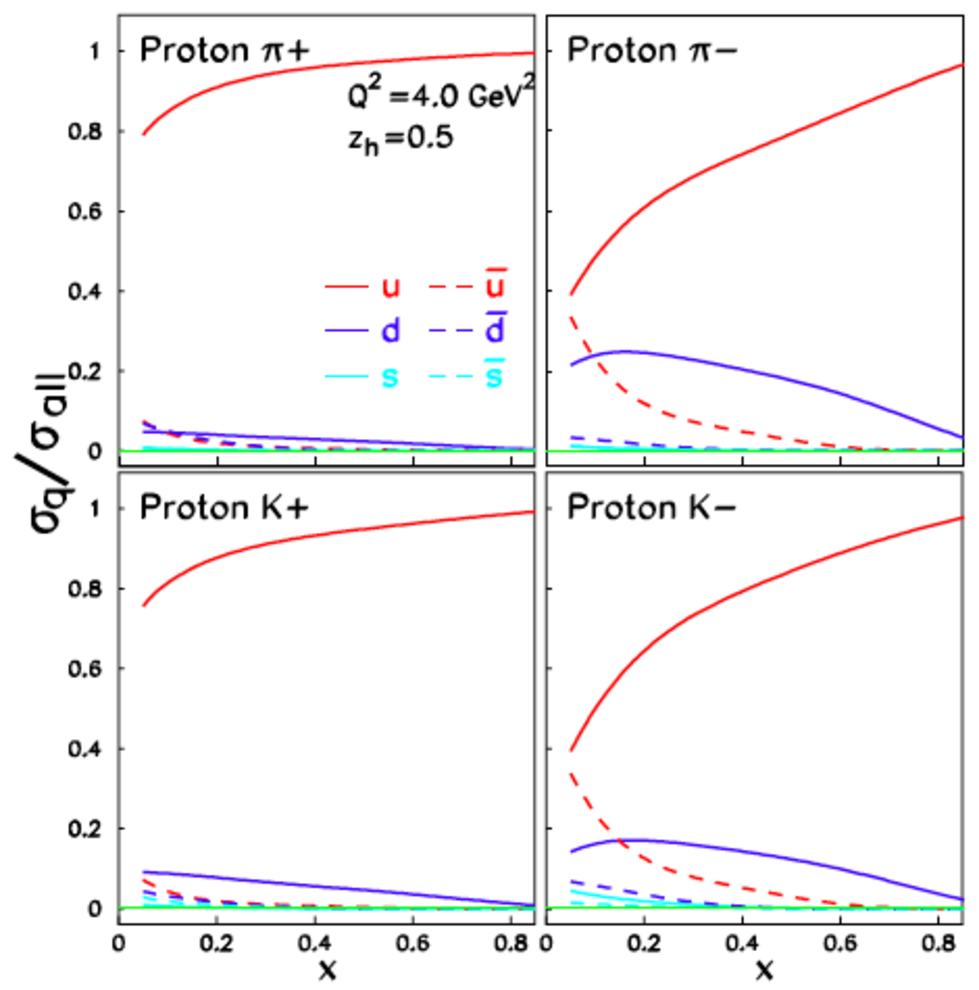
\includegraphics[width=0.51\linewidth]{figs_xj/crossq_ratio_proton_052014.pdf}
    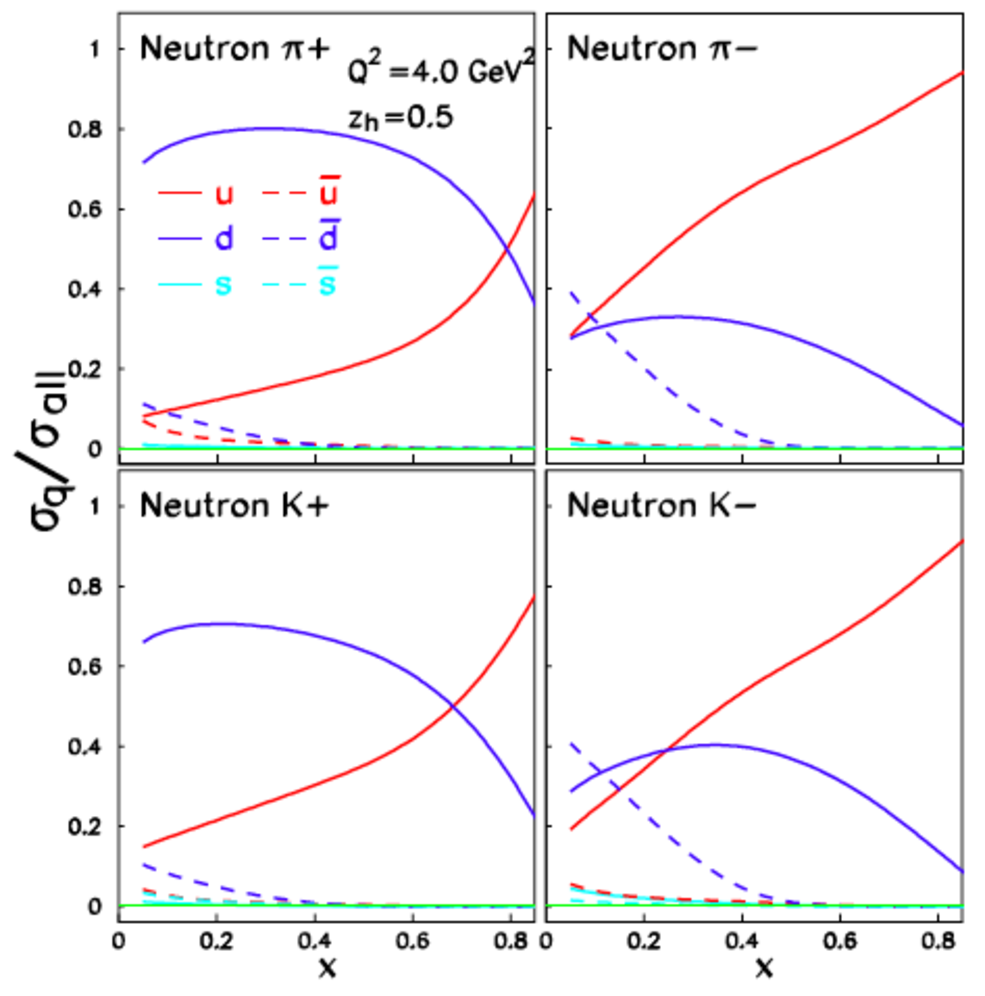
\includegraphics[width=0.51\linewidth]{figs_xj/crossq_ratio_neutron_052014.pdf} \\
\caption{\label{fig:crossq} The left panel shows the  
proton SIDIS cross sections as fractional contributions from 
each quark flavor at $Q^2=4.0$ GeV$^2$ and $z=0.5$.
The right panel shows the case for a neutron. 
}
\end{figure}
%-------------------------------------------------------------------------------

\section{SIDIS Cross sections at the next-to-leading order}


The naive $x$-$z$ separation is no longer valid at the next-to-leading order
when gluon diagrams in Fig.~\ref{fig:sidis} are considered. However, the exact form of 
the NLO cross section has been well-known~\cite{graudenz}. 
%%-------------------------------------------------------------------------------
\begin{figure}[htbp] 
~\hspace{0.25cm}LO:~\hspace{5.25cm} NLO-qq: \\
\vspace{-0.5cm} 
~\hspace{0.0cm}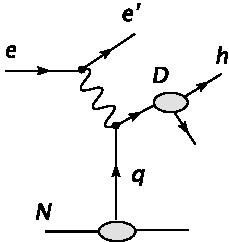
\includegraphics[width=0.24\linewidth]{figs_xj/lo1.pdf}
\hspace{2.0cm} 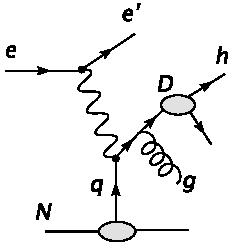
\includegraphics[width=0.24\linewidth]{figs_xj/nlo_qq1.pdf}
~~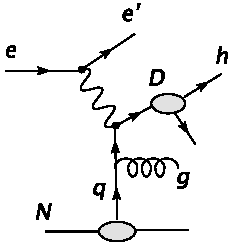
\includegraphics[width=0.25\linewidth]{figs_xj/nlo_qq2.pdf} \\
~ \\
~ \\
~\hspace{0.25cm}NLO-qg:~ \hspace{5.75cm} NLO-gq: \\
~\hspace{0.0cm}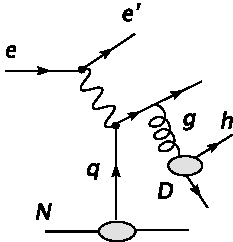
\includegraphics[width=0.24\linewidth]{figs_xj/nlo_qg1.pdf}
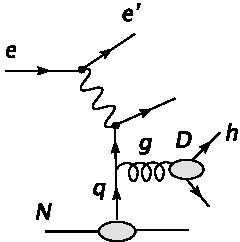
\includegraphics[width=0.24\linewidth]{figs_xj/nlo_qg2.pdf}
~\hspace{0.1cm}
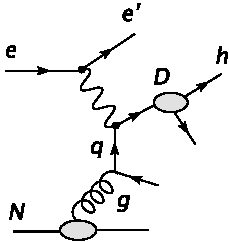
\includegraphics[width=0.24\linewidth]{figs_xj/nlo_gq1.pdf}
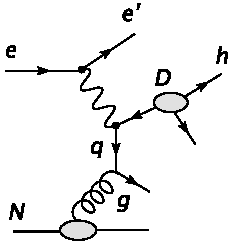
\includegraphics[width=0.24\linewidth]{figs_xj/nlo_gq2.pdf}
\caption{\label{fig:sidis} SIDIS diagrams at \lo (LO) and the \nlo (NLO).
}
\end{figure}
%-------------------------------------------------------------------------------
At NLO,  
the terms of $q(x)\cdot D(z)$ and $\Delta q(x) \cdot D(z)$ in Eq.~\ref{eq:fact} are added 
with the double convolutions of the type $q \otimes {\cal C} \otimes D$ and $\Delta q \otimes \Delta C \otimes D$
in which ${\cal C}$ and $\Delta C$ are well-known Wilson coefficients~\cite{wilson}: 
%The range of integration is 
%$x \le x^\prime \le 1$ and $z \le z^\prime \le 1$ for the current fragmentation~\cite{ssissakian2}.
%The double convolution is:
 \begin{eqnarray}
  [q \otimes C \otimes D](x,z)= \int_x^1 { dx^\prime \over x^\prime} \int_z^1 {d z^\prime \over z^\prime}
 q \left( {x \over x^\prime} \right) C(x^\prime, z^\prime) D \left( {z \over z^\prime} \right).
\label{eq:nlo}  
\end{eqnarray}
%Not only are $x$ and $z$ mixed through the double convolutions at the \nloo,
%the unpolarized cross section $\sigma^h$ also depends on the virtual photon variable 
%$y=(E_0-E^\prime)/E_0$ due to the longitudinal component of the virtual photon. 
 
We define the short-hand notation:
 \begin{eqnarray}
  qD + {\alpha_s \over 2 \pi} q \otimes C \otimes D = 
 q \left[ 1+ \otimes {\alpha_s \over 2 \pi} C \otimes \right] D,
\end{eqnarray}
at NLO instead of Eq.~\ref{eq:fact}, we have:
 \begin{eqnarray}
\label{Eq:nlo1}
\sigma^h(x,z) & = & \sum_{f}  e_f^2 q_f \left[ 1 + \otimes {\alpha_s \over 2 \pi} {\cal C}_{qq} \otimes \right] 
          D_{q_f}^{h}  \nonumber \\ 
& + & \left( \sum_{f}  e_f^2 q_f \right) \otimes {\alpha_s \over 2 \pi} {\cal C}_{qg} \otimes D_G^h
+ G \otimes {\alpha_s \over 2 \pi} {\cal C}_{gq} \otimes \left( \sum_{f} e_f^2 D_{q_f}^{h} \right),  \\
\label{Eq:nlo2}
\Delta \sigma^h(x,z) & = & \sum_{f}  e_f^2 \Delta q_f \left[ 1 + \otimes {\alpha_s \over 2 \pi} \Delta C_{qq} 
 \otimes \right] 
          D_{q_f}^{h}  \nonumber \\ 
& + & \left( \sum_{f}  e_f^2 \Delta q_f \right) \otimes {\alpha_s \over 2 \pi} \Delta C_{qg} \otimes D_G^h
+ \Delta G \otimes {\alpha_s \over 2 \pi} \Delta C_{gq} \otimes \left( \sum_{f} e_f^2 D_{q_f}^{h} \right).
\end{eqnarray}
%For any given form of the parton distributions,  the SIDIS cross sections can be calculated numerically~\cite{defs2000}
%according to Eq.~\ref{Eq:nlo1} and Eq.~\ref{Eq:nlo2}. 
It is also well-known that in the 
Mellin-$n$ space,
the double-convolutions factorize into simple products under moments, and the parton distributions 
can be recovered by an inverse Mellin transformation with all moments of Wilson
coefficients already calculated~\cite{stratmann2001}. 


\section{NLO global QCD analysis of DIS and SIDIS data}

At the \nloo, the cross sections in Eq.~\ref{Eq:a1h}  are replaced by Eq.~\ref{Eq:nlo1}
and Eq.~\ref{Eq:nlo2}. Following the well established~\cite{DSSV2008} formalism, 
tools of NLO QCD global fits,
which include data sets from inclusive and semi-inclusive reactions as well as $pp$ data,
have become available~\cite{DSSV2008}, and the uncertainties of the pPDF 
can be addressed in the global fits.
With the HERMES results, the polarized SIDIS data 
have a non-negligible weight in the combined global analysis, 
comparable to that of inclusive data. It helped 
to constrain the sea quark and gluon polarization complementing 
the information obtained from DIS.
The NLO global fit~\cite{DSSV2008} to the existing DIS and SIDIS data are shown in Fig.~\ref{fig:sasnlo} in Appendix. 
%Complete consistency between DIS and SIDIS asymmetries were found. However,
%when two different sets of fragmentation function Kretzer~\cite{kretzer} and KKP~\cite{kkp} parametrizations were used,
%noticeable differences were obtained on asymmetries (see Appendix). 
%This feature suggested that SIDIS data can also be used  
%to constrain fragmentation functions in conjunction with data from
%electron-positron annihilation.
%In Ref.~\cite{sassotnlo}, the profile of the $\chi^2$ function against different degrees 
%of polarization in each flavor were also explored such that uncertainties of the pPDFs were obtained.

The precision data from SIDIS spin asymmetry $A_{!N}^h$, especially adding the 
 neutron asymmetries such as from this experiment  to the world data,  
will serve as stringent constraints on pPDFs through NLO global fits, constraining sea quark polarization, and indirectly constrain gluon polarization $\Delta g(X)$, as shown through an earlier study for the JLab-6GeV case~\cite{Jiang:2006qc}.  
An ``impact study''' of the expected data from this experiment to the global NLO fit (DSSV++) is currently underway, the final results of the ``impact study'' will be presented at the PAC42 presentation.
%The impacts on pPDF moments are presented in the result section. 
Since the combined asymmetries $A_{1n}^{\pi^+ -\pi^-}$ 
are also measured in this experiment,  the result of the NLO global fit 
can be  cross checked with that from the NLO Christova-Leader method.

\section{Method of spin-flavor decomposition}
%Several independent  methods can be used to achieve 
% spin-flavor decomposition. 
%At \loo, the result from the LO Christova-Leader method will be cross 
%checked against  the ``fixed-$z$ purity'' method
%and the Monte Carlo purity method. 
%Within the same data set, 
%the naive $x$-$z$ \lo factorization assumption can be  
% tested quantitatively by comparing the combined asymmetry $A_{1n}^{\pi^+ + \pi^-}$ with the inclusive
%asymmetry $A_{1n}$.
%%Their differences will clearly demonstrate the size 
%%of the \lo factorization violation due to the \nlo contributions.
%%In this section, we give a brief outline of these flavor decomposition methods. 
%%More details are provided in Appendix.

\subsection{LO Christova-Leader method to obtain $\Delta u_v(x)$, $\Delta d_v(x)$ and $\Delta \bar{u}(x) - \Delta \bar{d}(x)$}
At the leading order, 
under isospin symmetry and charge conjugation invariance, the fragmentation functions 
cancel exactly in the combined asymmetry $A_{1N}^{\pi^+ \pm \pi^-}$. In addition, higher-twist 
terms in the fragmentation functions are also expected to be largely canceled~\cite{leader2}.
In the quantities related to $\sigma^{\pi^+} - \sigma^{\pi^-}$ which is a charge and flavor non-singlet
combination, sea-quarks and gluons do
not contribute at any QCD-order~\cite{leader2}.

From the Appendix, at \lo, for polarized 
protons, polarized deuterons and polarized neutrons~\footnote{After the effective neutron polarization ($86.5 \%$) 
in $^3$He is taken into account and the correction corresponding to the small 
proton polarization ($2.8 \%$) is applied.} (in $^3$He), we have:
\begin{eqnarray}
\label{eq:cllo}
&A&\hspace{-0.1cm}_{1p}^{\pi^+ - \pi^-}({\vec p})  =  { \Delta \sigma_p^{\pi^+}-\Delta \sigma_p^{\pi^-} \over
\sigma_p^{\pi^+} - \sigma_p^{\pi^-} }=
{  4\Delta u_v - \Delta d_v 
\over 4u_v - d_v }, \\
&A&\hspace{-0.1cm}_{1d}^{\pi^+ - \pi^-} ({\vec p}+ {\vec n}) =  { \Delta \sigma_d^{\pi^+}-\Delta \sigma_d^{\pi^-} \over
\sigma_d^{\pi^+}- \sigma_d^{\pi^-} }=
{ \Delta u_v + \Delta d_v 
\over u_v + d_v}, \\
&A&\hspace{-0.1cm}_{1He}^{\pi^+ - \pi^-} ({\vec n}+2p) =  { \Delta \sigma_{He}^{\pi^+}-\Delta \sigma_{He}^{\pi^-} \over
\sigma_{He}^{\pi^+}- \sigma_{He}^{\pi^-} }=
{ 4\Delta d_v - \Delta u_v 
\over 7 u_v + 2 d_v}. 
\end{eqnarray}
Measurements on three different targets will over-determine $\Delta u_v$ and $\Delta d_v$.
Proton and deuteron measurements are more sensitive to $\Delta u_v$, measurements on $^3$He  
are more sensitive
to $\Delta d_v$. One can re-write the last relation as:
\begin{eqnarray}
\label{Eq:cl2}
%&(\Delta u_v)_{LO}&  = {1 \over 5} \left[ \left( 4u_v - d_v)\cdot  A_{1p}^{\pi^+ - \pi^-}
%                 + (u_v + d_v) \cdot A_{1d}^{\pi^+ - \pi^-} \right) \right],  \\
&(\Delta d_v-{1 \over 4} \Delta u_v )_{LO} &  = {1 \over 4} \left( 7 u_v + 2 d_v \right)  A_{1He}^{\pi^+ - \pi^-}.
\end{eqnarray}
This method of flavor decomposition involves helicity asymmetries of cross section differences. 
Kinematics need to be carefully chosen 
such that $\pi^+$ and $\pi^-$ cross sections are reasonably different.  
Error propagation on $A_{1N}^{\pi^+ - \pi^-}$ make this method unfavorable when $\pi^-/\pi^+$ ratio
approaches unity. Fig.~\ref{fig:hermescl}  in Appendix illustrates this point by comparing the purity method with
the Christova-Leader method for HERMES data~\cite{hermesthesis}.

We can obtain the \lo quantity 
$\Delta u_v - \Delta d_v$ from combinations of either proton and $^3$He data or proton and deuteron data as:
\begin{eqnarray}
\label{Eq:uvdv}
&(\Delta u_v - \Delta d_v)_{LO}&  = {1 \over 5} \left[  \left( 4u_v - d_v)  
A_{1p}^{\pi^+ - \pi^-} 
                 -  (7u_v + 2 d_v) A_{1He}^{\pi^+ - \pi^-} \right) \right], \\ 
&(\Delta u_v - \Delta d_v)_{LO}&  = {1 \over 5} \left[ 2 \left( 4u_v - d_v)  
A_{1p}^{\pi^+ - \pi^-} 
                 -3  (u_v + d_v) A_{1d}^{\pi^+ - \pi^-} \right) \right]. 
\end{eqnarray}

On the other hand, constrained by the inclusive data, the flavor non-singlet quantity at all QCD orders is:
\begin{equation}
\label{Eq:cl3}
\Delta q_3(x,Q^2) \equiv (\Delta u + \Delta \bar{u}) - (\Delta d + \Delta \bar{d}).
\end{equation}
The polarized sea asymmetry at all QCD orders is:
\begin{equation}
 \Delta \bar{u} - \Delta \bar{d} = {1 \over 2}\Delta q_3 - {1 \over 2}(\Delta u_v - \Delta d_v).
\end{equation}


At the leading order, we have:
\begin{equation}
\Delta q_3(x,Q^2) \vert_{LO} = 6 \left[ g_1^p(x,Q^2) - g_1^n(x,Q^2) \right],
\end{equation}
\begin{eqnarray}
\label{Eq:cl4}
\left[\Delta \bar{u}(x) - \Delta \bar{d}(x) \right]_{LO} & = & 3 \left[ g_1^p(x)- g_1^n(x)) \right] 
 - {1 \over 2} (\Delta u_v - \Delta d_v) \vert_{LO}.
% & = & 3 \left[ g_1^p(x)- g_1^n(x)) \right] - {3 \over 8}\Delta u_v (x) \vert_{LO} \nonumber \\ 
% &   & +  {1 \over 8} \left( 7 u_v (x)+ 2 d_v (x) \right) 
%\cdot  A_{1He}^{\pi^+ - \pi^-}(x). 
\end{eqnarray}
%A similar relation holds at the \nloo.

\subsection{NLO Christova-Leader method}
At the \nloo, under isospin symmetry and charge conjugation invariance, 
the NLO convolution terms become much simpler in quantities that 
are related to $\sigma^{\pi^+} - \sigma^{\pi^-}$. Since the gluon-related terms  
  are identical for  
$\pi^+$ and $\pi^-$ production, they drop out in the differences~\cite{leader2}:
 \begin{eqnarray}
\label{Eq:a1pnlo}
A_{1p}^{\pi^+ - \pi^-}({\vec p}) & = &  { (4 \Delta u_v -\Delta d_v) \left[ 1+ \otimes (\alpha_s/2\pi) \Delta C_{qq}
\otimes \right] (D^+ -D^-) \over { (4 u_v - d_v) \left[ 1+ \otimes (\alpha_s/2\pi) {\cal C}_{qq}
\otimes \right] (D^+ - D^-) } },  \\ 
A_{1d}^{\pi^+ - \pi^-}({\vec p}+ {\vec n}) & = &  { (\Delta u_v + \Delta d_v) \left[ 1+ \otimes (\alpha_s/2\pi) \Delta C_{qq}
\otimes \right] (D^+ -D^-)  \over { (u_v + d_v) \left[ 1+ \otimes (\alpha_s/2\pi) {\cal C}_{qq}
\otimes \right] (D^+ -D^-) } },  \\
A_{1He}^{\pi^+ - \pi^-}({\vec n}+2p) & = &  { (4 \Delta d_v - \Delta u_v) \left[ 1+ \otimes (\alpha_s/2\pi) \Delta C_{qq}
\otimes \right] (D^+ -D^-)  \over { (7 u_v + 2 d_v) \left[ 1+ \otimes (\alpha_s/2\pi) {\cal C}_{qq}
\otimes \right] (D^+ -D^-) } }.
\end{eqnarray}
in which $\Delta u_v$ and $\Delta d_v$ evolve as non-singlets and do not mix with 
sea-quark and gluon densities. Therefore, measurements of $A_{1N}^{\pi^+ - \pi^-}$ 
can determine $\Delta u_v$ and $\Delta d_v$ at the next-to-leading order
without any consideration of gluon and sea distributions.
The double-convolution terms in Eq.~\ref{Eq:a1pnlo} are expected to introduce negligible
$z$-dependency in $A_{1N}^{\pi^+ - \pi^-}$ at the kinematics of this experiment, 
as demonstrated in calculation of de Florian, Navarro and Sassot~\cite{sassotnlo}.
%The solution of Eq.~\ref{Eq:a1pnlo} would follow an iterative procedure
% with the order from higher-$x$ to lower-$x$ points, 
%since $\Delta q_v$ at higher-$x$ feed into the solution of 
% lower-$x$ in the convolution terms.
%Initial assumptions of $\Delta q_v$ at high-$x$
%can be taken from a theoretical ansatz that respects positivity limits. 

The first moment of $\Delta u_v - \Delta d_v$ is related to the moment 
of $\Delta \bar{u} -\Delta \bar{d}$ through the Bjorken sum rule at all orders of QCD~\cite{ssissakian2}.
The Bjorken sum rule, written in terms of 
the moment $\Delta_1 q=\int_0^1dx \Delta q$,
\begin{eqnarray}
\label{Eq:bsr1}
\Delta_1 q_3 & \equiv & \left[ \Delta_1 u(Q^2)+ \Delta_1 \bar{u}(Q^2) \right] - 
\left[ \Delta_1 d(Q^2)+ \Delta_1 \bar{d}(Q^2) \right] \nonumber \\
 & =& \left| {g_A \over g_v} \right| =1.2670 \pm 0.0035 ~~valid~~ in ~ all ~ QCD ~ orders. 
\end{eqnarray}
Therefore, valid in all QCD orders, we have:
\begin{eqnarray}
\label{Eq:bsr2}
\int_0^1(\Delta \bar{u}  - \Delta \bar{d})dx = {1 \over 2} \left| {g_A \over g_v} \right|
- {1 \over 2} \int_0^1(\Delta {u_v}  - \Delta {d_v} )dx.
\end{eqnarray}
%
In other words, if one  measures the valence quark moment $\Delta {u_v}  - \Delta {d_v}$ precise enough, for example to 
$\delta \left[ \Delta_1 u_v - \Delta_1 d_v \right] = \pm 0.05$,  
one cam pin down the polarized sea asymmetry, to $\delta \left[ \Delta_1 \bar{u} - \Delta_1 \bar{d} \right] = \pm 0.025$, that's 
 eight standard deviations from the prediction of Chiral Quark Soliton model.

A well-defined procedure has been given~\cite{ssissakian2}
 to obtain the moment $\Delta_1 {u_v}  - \Delta_1 {d_v}$ directly
 from the measured asymmetries $A_{1N}^{\pi^+ - \pi^-}$ without 
first solving Eq.~\ref{Eq:a1pnlo} point-to-point. 
The stability of this procedure has been demonstrated~\cite{ssissakian2}
using the HERMES-1999 data.

From the deuteron data alone, one can also form $\Gamma_v$, the first moment of $\Delta u_v + \Delta d_v$, and extract
at \lo the moment:

\begin{equation}
 \int_0^1 (\Delta \bar{u} +\Delta \bar{d})dx = 3 \Gamma_1^N -{1 \over 2}\Gamma_v+{1 \over 12} a_8 
\end{equation}
where $\Gamma_1^N$ is the moment of$g_1^N=(g_1^p+g_1^n)/2$ from inclusive data, and $a_8=3F-D$ is from hyperon $\beta$-decays.

The  COMPASS deuteron target results~\cite{compass2007} of $A_d^{h^+ - h^-}$ are shown in Fig.~\ref{fig:compass2}. The extracted valence
quark polarization $x(\Delta u_v + \Delta d_v)$ and the running-$x_{min}$ integral of $\Delta u_v + \Delta d_v$ are 
shown in Fig.~\ref{fig:compass3}.  The fact that the integral of $\Delta u_v + \Delta d_v$ is significantly different from that of 
assumption of a symmetrical polarized sea indicated that the sign of $\Delta \bar{u}$ is opposite to that of $\Delta \bar{d}$.       

%-------------------------------------------------------------------------------
\begin{figure}[tbhp]
\centerline{
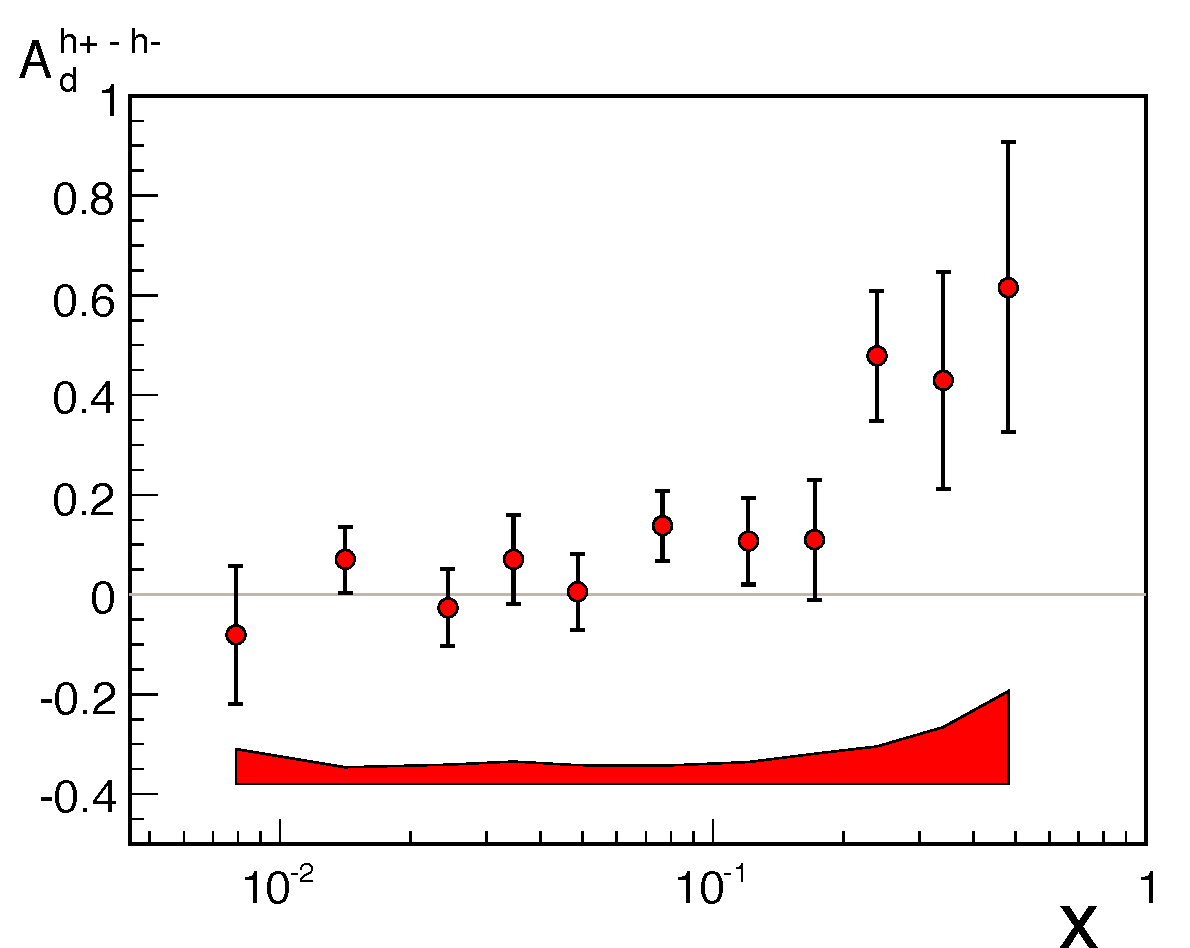
\includegraphics[width=0.70\linewidth]{figs_xj/compass_korzenev_Adiff.pdf}
}
\caption{\label{fig:compass2} Charged hadron combined asymmetry $A_d^{h^+ - h^-}$ measured by COMPASS~\protect\cite{compass2007}.
}
\end{figure}
%-------------------------------------------------------------------------------

%-------------------------------------------------------------------------------
\begin{figure}[tbhp]
\centerline{
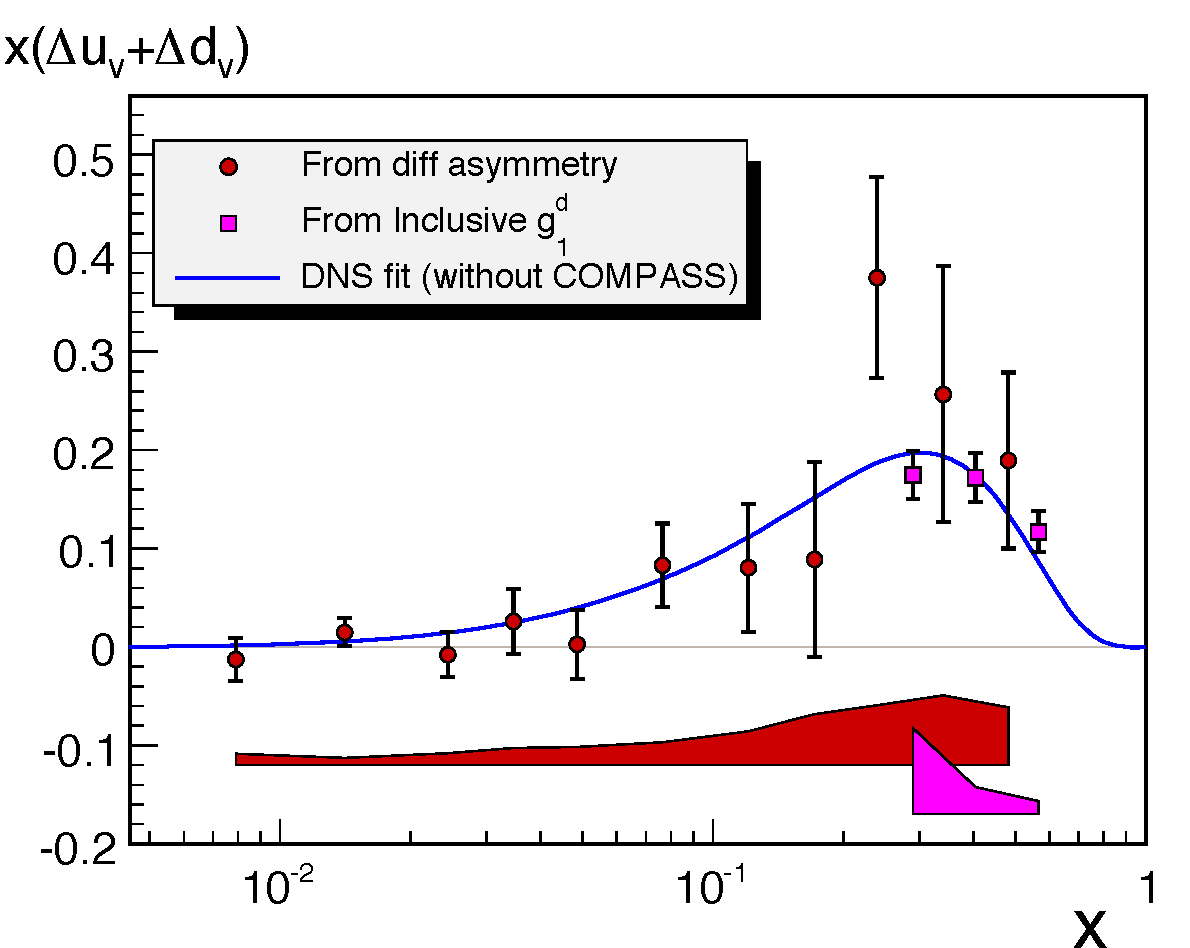
\includegraphics[width=0.50\linewidth]{figs_xj/compass_korzenev_udv.pdf}
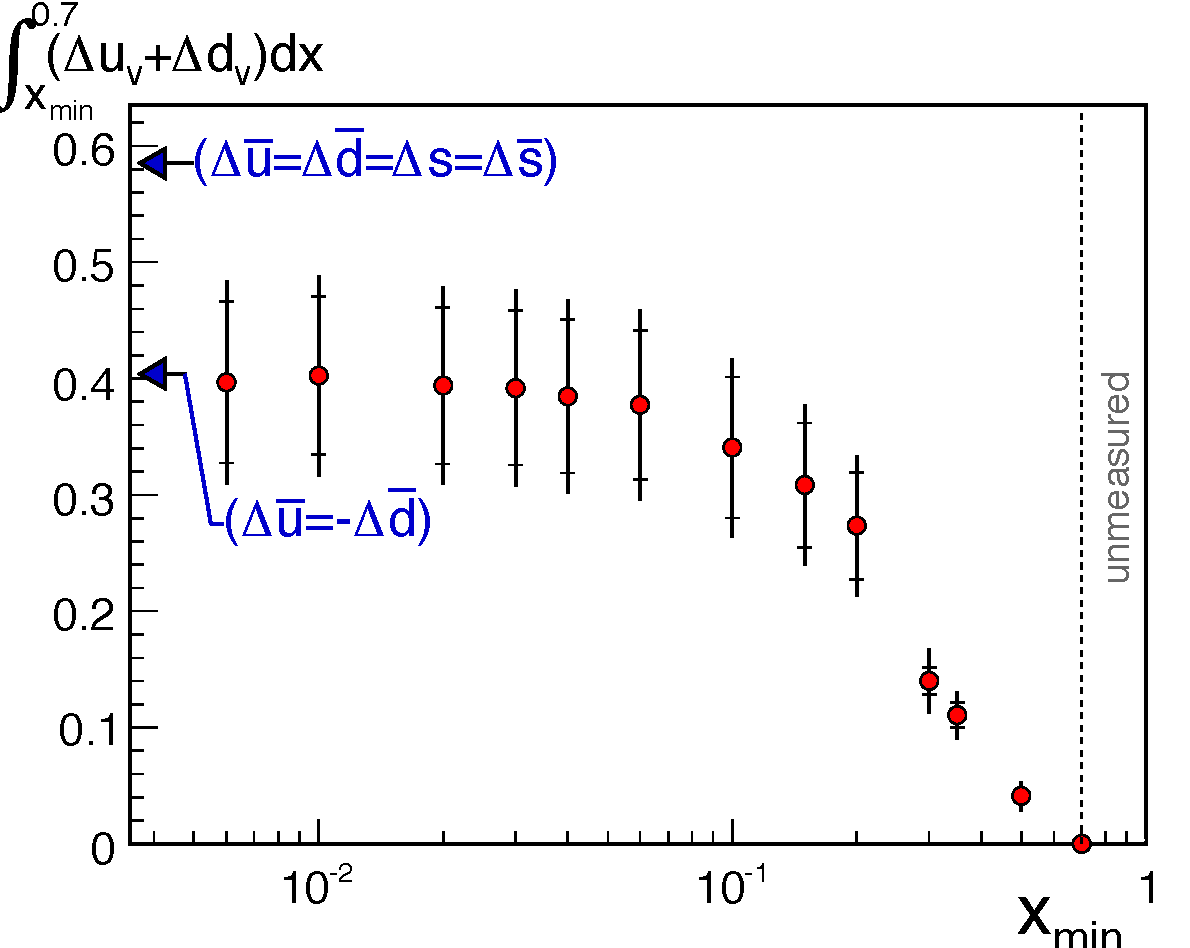
\includegraphics[width=0.50\linewidth]{figs_xj/compass_korzenev_int.pdf}
}
\caption{\label{fig:compass3} The valence
quark polarization $x(\Delta u_v + \Delta d_v)$ compared with fron that of inclusive $g_1^d$ data, and the running-$x_{min}$ 
integral of $\Delta u_v + \Delta d_v$ from the deuteron data of COMPASS~\protect\cite{compass2007} at $Q^2=10$ GeV$^2$.
}
\end{figure}
%-------------------------------------------------------------------------------

\subsection{Cross check $\Delta q_v$ with measurement at RHIC}

At RHIC,  $\Delta q$ can be measured through 
$W^\pm$ decays~\cite{bunce00}.  Since the $Q^2$-evolutions of valence densities  $\Delta q_v$ 
are well understood in QCD, consistency cross checks can be made between JLab data at $\langle Q^2 \rangle=4.0$ GeV$^2$
and RHIC data at $Q^2 = M_W^2$.   

\subsection{Spin observables to check the \lo naive $x$-$z$ separation}

A schematic strategy of to test \lo naive $x$-$z$ separation
was suggested \cite{leader2} which requires prior knowledge of neither fragmentation functions nor
parton distributions. The experimental observables in this strategy
is to make the combined double-spin asymmetry $A_{1N}^{\pi^+ + \pi^-}$. 
If \lo naive $x$-$z$ separation holds perfectly, 
$A_{1N}^{\pi^+ + \pi^-}$ will turn out to be identical to the inclusive 
$A_{1N}$ asymmetry due to the exact
 cancellation of the fragmentation functions in the asymmetry 
under charge conjugation invariance and isospin symmetry.
Their difference, $A_{1N}^{\pi^+ + \pi^-}-A_{1N}$, gives a clear indication 
on the size of the next-to-leading-order terms which violate the naive \lo 
$x$-$z$ separation.

Assume $\Delta s = \Delta \bar{s} \approx 0$, 
 the fragmentation functions are canceled at the leading order in 
 the combined asymmetry $A_{1N}^{\pi^+ + \pi^-}$, such that: 

\begin{eqnarray}
\label{Eq:a1pp1}
&A&\hspace{-0.1cm}_{1p}^{\pi^+ + \pi^-} (x,Q^2,z) =  { \Delta \sigma_p^{\pi^+}+\Delta \sigma_p^{\pi^-} \over
\sigma_p^{\pi^+}+ \sigma_p^{\pi^-} }=
{  4(\Delta u+ \Delta \bar{u}) + \Delta d + \Delta \bar{d} 
\over 4(u  + \bar {u}) + d+ \bar{d}  } \equiv A_{1p}(x,Q^2),  \nonumber \\
&A&\hspace{-0.1cm}_{1d}^{\pi^+ + \pi^-}(x,Q^2,z) ={ \Delta \sigma_d^{\pi^+}+\Delta \sigma_d^{\pi^-} \over
\sigma_d^{\pi^+}+ \sigma_d^{\pi^-} }=  
{  \Delta u+\Delta d + \Delta \bar{u}+ \Delta \bar{d}
\over u +d + {\bar u}+ {\bar d} } \equiv A_{1d}(x,Q^2),  \nonumber \\ 
&A&\hspace{-0.1cm}_{1n}^{\pi^+ + \pi^-}(x,Q^2,z) ={ \Delta \sigma_{n}^{\pi^+}+\Delta \sigma_{n}^{\pi^-} \over
\sigma_{n}^{\pi^+}+ \sigma_{n}^{\pi^-} }=  
{  \Delta u + \Delta \bar{u}+ 4(\Delta d + \Delta \bar{d})
\over u + {\bar u}+  4(d + {\bar d}) } \equiv A_{1n}(x,Q^2). 
\end{eqnarray}
The combined asymmetry $A_{1N}^{\pi^+ + \pi^-}$ 
reduces to the inclusive asymmetry $A_{1N}$ under the \lo naive $x$-$z$ separation. 
The relation 
$A_{1N}^{\pi^+ + \pi^-}(x,Q^2,z) = A_1(x,Q^2)$ is a rather strong condition to satisfy, 
since the left-hand side involves the hadron observable $z$ while the right-hand side
doesn't.  The deviation of $A_{1N}^{\pi^+ + \pi^-}$ from the inclusive $A_{1N}$ asymmetry
``effectively'' measures the relative importance of the contribution from the \nlo terms.

%%------------------------------------------------------------------------------
%\begin{figure}[htbp] 
%\centerline{{\epsfig{figure=plots/hermes_A1-inc-h+h-.eps,height=65mm}} 
%} 
%\vspace{-5.0mm}
%\caption{\label{fig:hermesc} 
%The HERMES inclusive asymmetries on the proton and the deuteron are compared with 
%the respective semi$-$inclusive combined $h^+ + h^-$ asymmetries. 
%The top panels show the asymmetries, where the hadron tagged asymmetry is offset in $x$ 
%for presentation. The lower panel shows the ratio of the uncertainties,  
%$\delta(A_1)/\delta(A_{1N}^{h^+ +h^-})$.
%}
%\end{figure} 
%%------------------------------------------------------------------------------
The HERMES experiment extracted the combined asymmetry $A_{1N}^{h + \bar{h}}$ as shown in 
Fig.~\ref{fig:hermesc} in comparison with the inclusive asymmetry $A_{1N}$.
The near perfect agreement of $A_{1N}^{h + \bar{h}}$ with $A_{1N}$ at $\langle Q^2 \rangle =2.5$ GeV$^2$ 
indicated that the \nlo correction terms are small or mostly canceled 
in the asymmetries and the target fragmentation contribution has a negligible impact to the asymmetries. 
Even better agreements should be expected in this experiment at JLab-12GeV, since the much higher luminosity allow 
reasonable statistics at larger scattering angle resulted in $\langle Q^2 \rangle =4.0$ GeV$^2$ for this experiment.
Once this agreement can be clearly demonstrated with high precision,
parton polarizations can be reliably extracted through the \lo interpretation of SIDIS asymmetries.  

%\subsubsection{Effects of higher-twist in semi-inclusive asymmetries}
%It was shown explicitly that higher twist effect in inclusive asymmetries are consistent with zero.
%(Leader+Stamenov).
